\documentclass[a4paper]{report}

\setcounter{tocdepth}{4}
\setcounter{secnumdepth}{3}

\usepackage{longtable}
\usepackage{comment}
\usepackage{multirow}
\usepackage[utf8]{inputenc}
\usepackage[T1]{fontenc}
\usepackage[pdftex]{graphicx}
\usepackage{xcolor}
	\definecolor{myGreen}{rgb}{0,1,0.85}
%\usepackage[capposition=top]{floatrow}   
% \usepackage[margin=1in]{geometry} 
\usepackage{subfigure}

\usepackage[english]{babel} 
\usepackage{algorithmicx}
\usepackage{algpseudocode}

\usepackage{amsmath}
\usepackage{amssymb}
\usepackage{amsthm}
\DeclareMathOperator{\Tr}{Tr}
\usepackage{bigints}

%\usepackage{subcaption}

\usepackage{titlesec}
\newcommand{\sectionbreak}{\clearpage}
\usepackage{lmodern}
\graphicspath{{../img/}}

 \DeclareGraphicsExtensions{.pdf,.jpg,.png}
\usepackage{microtype}


\usepackage[hidelinks,plainpages=false,pageanchor=false]{hyperref}
%\hypersetup{pageanchor=false}
\begin{document}


\begin{titlepage}
\begin{center}

% Upper part of the page. The '~' is needed because \\
% only works if a paragraph has started.


\textsc{\LARGE Singularity Graph Build}\\[1.5cm]

\textsc{\Large Report}\\[0.5cm]

% Title

{ \huge \bfseries Detailed draft and explanations \\[0.4cm] }



% Author and supervisor
\begin{minipage}{0.4\textwidth}
\begin{flushleft} \large
%\emph{Ph.D.:}\\
Ana-Maria \textsc{Vintescu}
\end{flushleft}
\end{minipage}
\begin{minipage}{0.4\textwidth}
\begin{flushright} \large
Franck \textsc{Ledoux}
\end{flushright}
\end{minipage}


% Bottom of the page
\date{} % blank date

\end{center}
\end{titlepage}


\date{} % blank date



\renewcommand{\thesection}{\arabic{section}}




\begin{abstract}
%\renewcommand{\thefootnote}{\arabic{footnote}}
 {Having as input a triangular mesh $M$ and an associated cross field $CF$ (one cross per vertex), we proceed to constructing a block-structured mesh whose blocks are ideally detected as portions of the mesh where the directions of the field are similar.
 \newline
 In a pre-processing step we compute and store the triangle centers $T_c$ and the crosses associated to them $CF[T_c]$ (\textcolor{blue}{$constructCenterTriangleCrosses()$}). 
 Also, using the function \textcolor{blue}{$computeFace2FaceInfo()$} we compute and store several values associated to faces or vertices of the mesh:
 \begin{itemize}
 \item \textcolor{myGreen}{$face\_normals$} - for each face, the normal is constructed
 \item \textcolor{myGreen}{$face2Face\_neighbours$} - for each face, the list of adjacent faces by edge is constructed
 \item \textcolor{myGreen}{$face2Face\_neighbours\_by\_verts$} - for each face, the list of adjacent faces by vertex is constructed
 \item \textcolor{myGreen}{$face2FaceTransport$} - for each face, for each of its \textcolor{myGreen}{$face2Face\_neighbours$} (in the same order), a value indicating the "transport" is computed (the angle obtained when transporting a vector from one reference frame to another)
 \item \textcolor{myGreen}{$face2FaceDeviation$} - for each face, for each of its \textcolor{myGreen}{$face2Face\_neighbours$} (in the same order), a value indicating the deviation of the cross field in between the triangle centers
 \item \textcolor{myGreen}{$is\_bdry\_face$} - boolean value indicating for each face if it has at least one vertex on the boundary.
 \item \textcolor{myGreen}{$bdry\_edge\_normals$} - for each boundary edge, the normal is constructed
 \item \textcolor{myGreen}{$bdry\_node\_normals$} - for each boundary vertex, the normal is constructed
 \item \textcolor{myGreen}{$newNode2NewNodeNeighbours$} - assuming a new mesh where the vertices are the vertices of the original mesh plus the vertices associated to all the triangle centers of the original mesh, construct the adjacency node to node.
 \end{itemize} 

 We proceed by detecting the singular triangles (\textcolor{blue}{$detectSingularTriangles()$}) and their degree (3 or 5-degree) and we compute the singular points locations and their slots' directions (\textcolor{blue}{$createSingPointAndSlots()$}).
 \newline
 However, if the user wants to prescribe certain singularity triangles (the singularity points are placed at the center of the triangles) by providing their ID, this is possible by setting \textcolor{myGreen}{$testPrescribedSing = true$}.  
 \newline
 For each interior boundary (surfaces with holes) we create an artificial point. 
 \newline
 If the user has chosen so \newline(\textcolor{myGreen}{$m\_build\_geometric\_singularities = true$}), we will also build the geometric singularities (\newline(\textcolor{blue}{$buildGeometricSlots()$})).
\newline
Further initialize the confusing balls around each singularity; a list of triangles whose centers are within a given distance (\textcolor{myGreen}{$m\_confusing\_distance = ATolerance*m\_mesh\_radius;$}) from the singularity. This value increases until we detect at least one triangle.
\newline
Further the actual strategy is implemented;
The user has chosen one of the following strategies:
\begin{itemize}
\item \textcolor{cyan}{$AStrategy==original$}
\newline
In this strategy, we depart iteratively from the singularity points along the slots directions, propagating the line using the Heun strategy (\textcolor{blue}{$computeStreamLine()$}) until reaching:
\begin{itemize}
\item the boundary
\item the confusing ball of a different singularity (are situated within \textcolor{myGreen}{
$m\_confusing\_distance$} from the singularity point).
\end{itemize}
\item \textcolor{cyan}{$AStrategy==simultaneousStartHeun$}
\newline
In this strategy, we depart simultaneously from all the singularity points along all the slots directions, propagating the line using the Heun strategy (\textcolor{blue}{$computeStreamLine()$}) until reaching:
\begin{itemize}
\item the boundary
\item within a prescribed distance from the ending point of a different streamline (set as 
\textcolor{myGreen}{$thresholdStreamLineDist = 100*mean\_edge\_length*ATolerance;$})
\item the confusing ball of a different singularity (unlikely).
\end{itemize}
\item \textcolor{cyan}{$AStrategy==simultaneousStartRK4$}
\newline
Same as above, except the propagation procedure is done using Runge-Kutta 4  (\textcolor{blue}{$growLineRK4()$}).
\item \textcolor{cyan}{$AStrategy==shortestPaths$}
\newline
For each slot we will try to detect the "shortest path" towards all other slots. Each of these possible streamlines will be the variables of an optimization procedure.

\end{itemize}
 
 }
\end{abstract}




\tableofcontents{}

\setcounter{tocdepth}{4}
\newpage
\section{Introduction}

{
 \textcolor{myGreen}{$Using\ this\ color\ we\ will\ denote\ variables\ from\ our\ code.$}
 
  \textcolor{blue}{$Using\ this\ color\ we\ will\ denote\ functions\ from\ our\ code.$}
}

\bigskip
\subsection{Motivation}

{
Motivation
%\begin{figure}[H]
%\includegraphics[width=0.5\textwidth]{img/mesh_completion.png}
%\caption{Mesh Completion \cite{KraevoyS05}}
%\floatfoot{Completing a head: (a,d) the input mesh, (b,e) the template, (d,f) the completed model}
%\end{figure}


%\begin{figure}[H]
%\includegraphics[width=0.9\textwidth]{img/remesh-cpcr.png}
%\caption{Remeshing \cite{Kraevoy2004}}
%\floatfoot{a) source mesh, b) target mesh after initial projection, c) smoothing step, d) final mesh}
%\end{figure}

}

\bigskip
\subsection{Definitions}
{  Definitions/Preliminaries

The input surface $M$ is given as a triangular 
mesh having a set of vertices $({M_V})$, edges $({M_E})$ and triangles $({M_T})$.
Their number is noted with $|M_V|$, $|M_E|$ and $|M_T|$ respectively.
The geometry of $M$ is given as the 3D coordinates of the vertices $X_{M_v}=({{M_v}_x},{{M_v}_y},{{M_v}_z}), \forall v\in{M_V}$. 


}

\newpage
\section{Section}
{ Section
\begin{comment}

\begin{equation}
J_f=U \Sigma V^T = U  \begin{pmatrix}
\sigma_1 & 0  \\
0 & \sigma_2 \\
0 & 0
\end{pmatrix} V^T
\end{equation}
\end{comment}

}


\newpage
\section{Discrete Strategy}
{
Initially we have the triangular mesh $(M \rightarrow (M_V, M_E, M_T))$. We also have a set of singularity points (detected as the critical points of a frame field associated to $M$): $S_{Pnts} = \{S_i = \{{S_i}_x, {S_i}_y, {S_i}_z \}; i=\overline{0,N}\}$, each of them having a set of slots: $S_{slots} = \{(S_{slots}^{points} , S_{slots}^{dir})\} = \{(S_i^j, \overrightarrow{S_i^j } ), S_i^j =\{{S_i^j}_x, {S_i^j}_y, {S_i^j}_z \},  \overrightarrow{S_i^j} = \overrightarrow{S_i,S_i^j } ; i=\overline{0,N} , j=\overline{0,4}\}$, Fig.~\ref{fig:singSlots}. 
\begin{figure}[h]
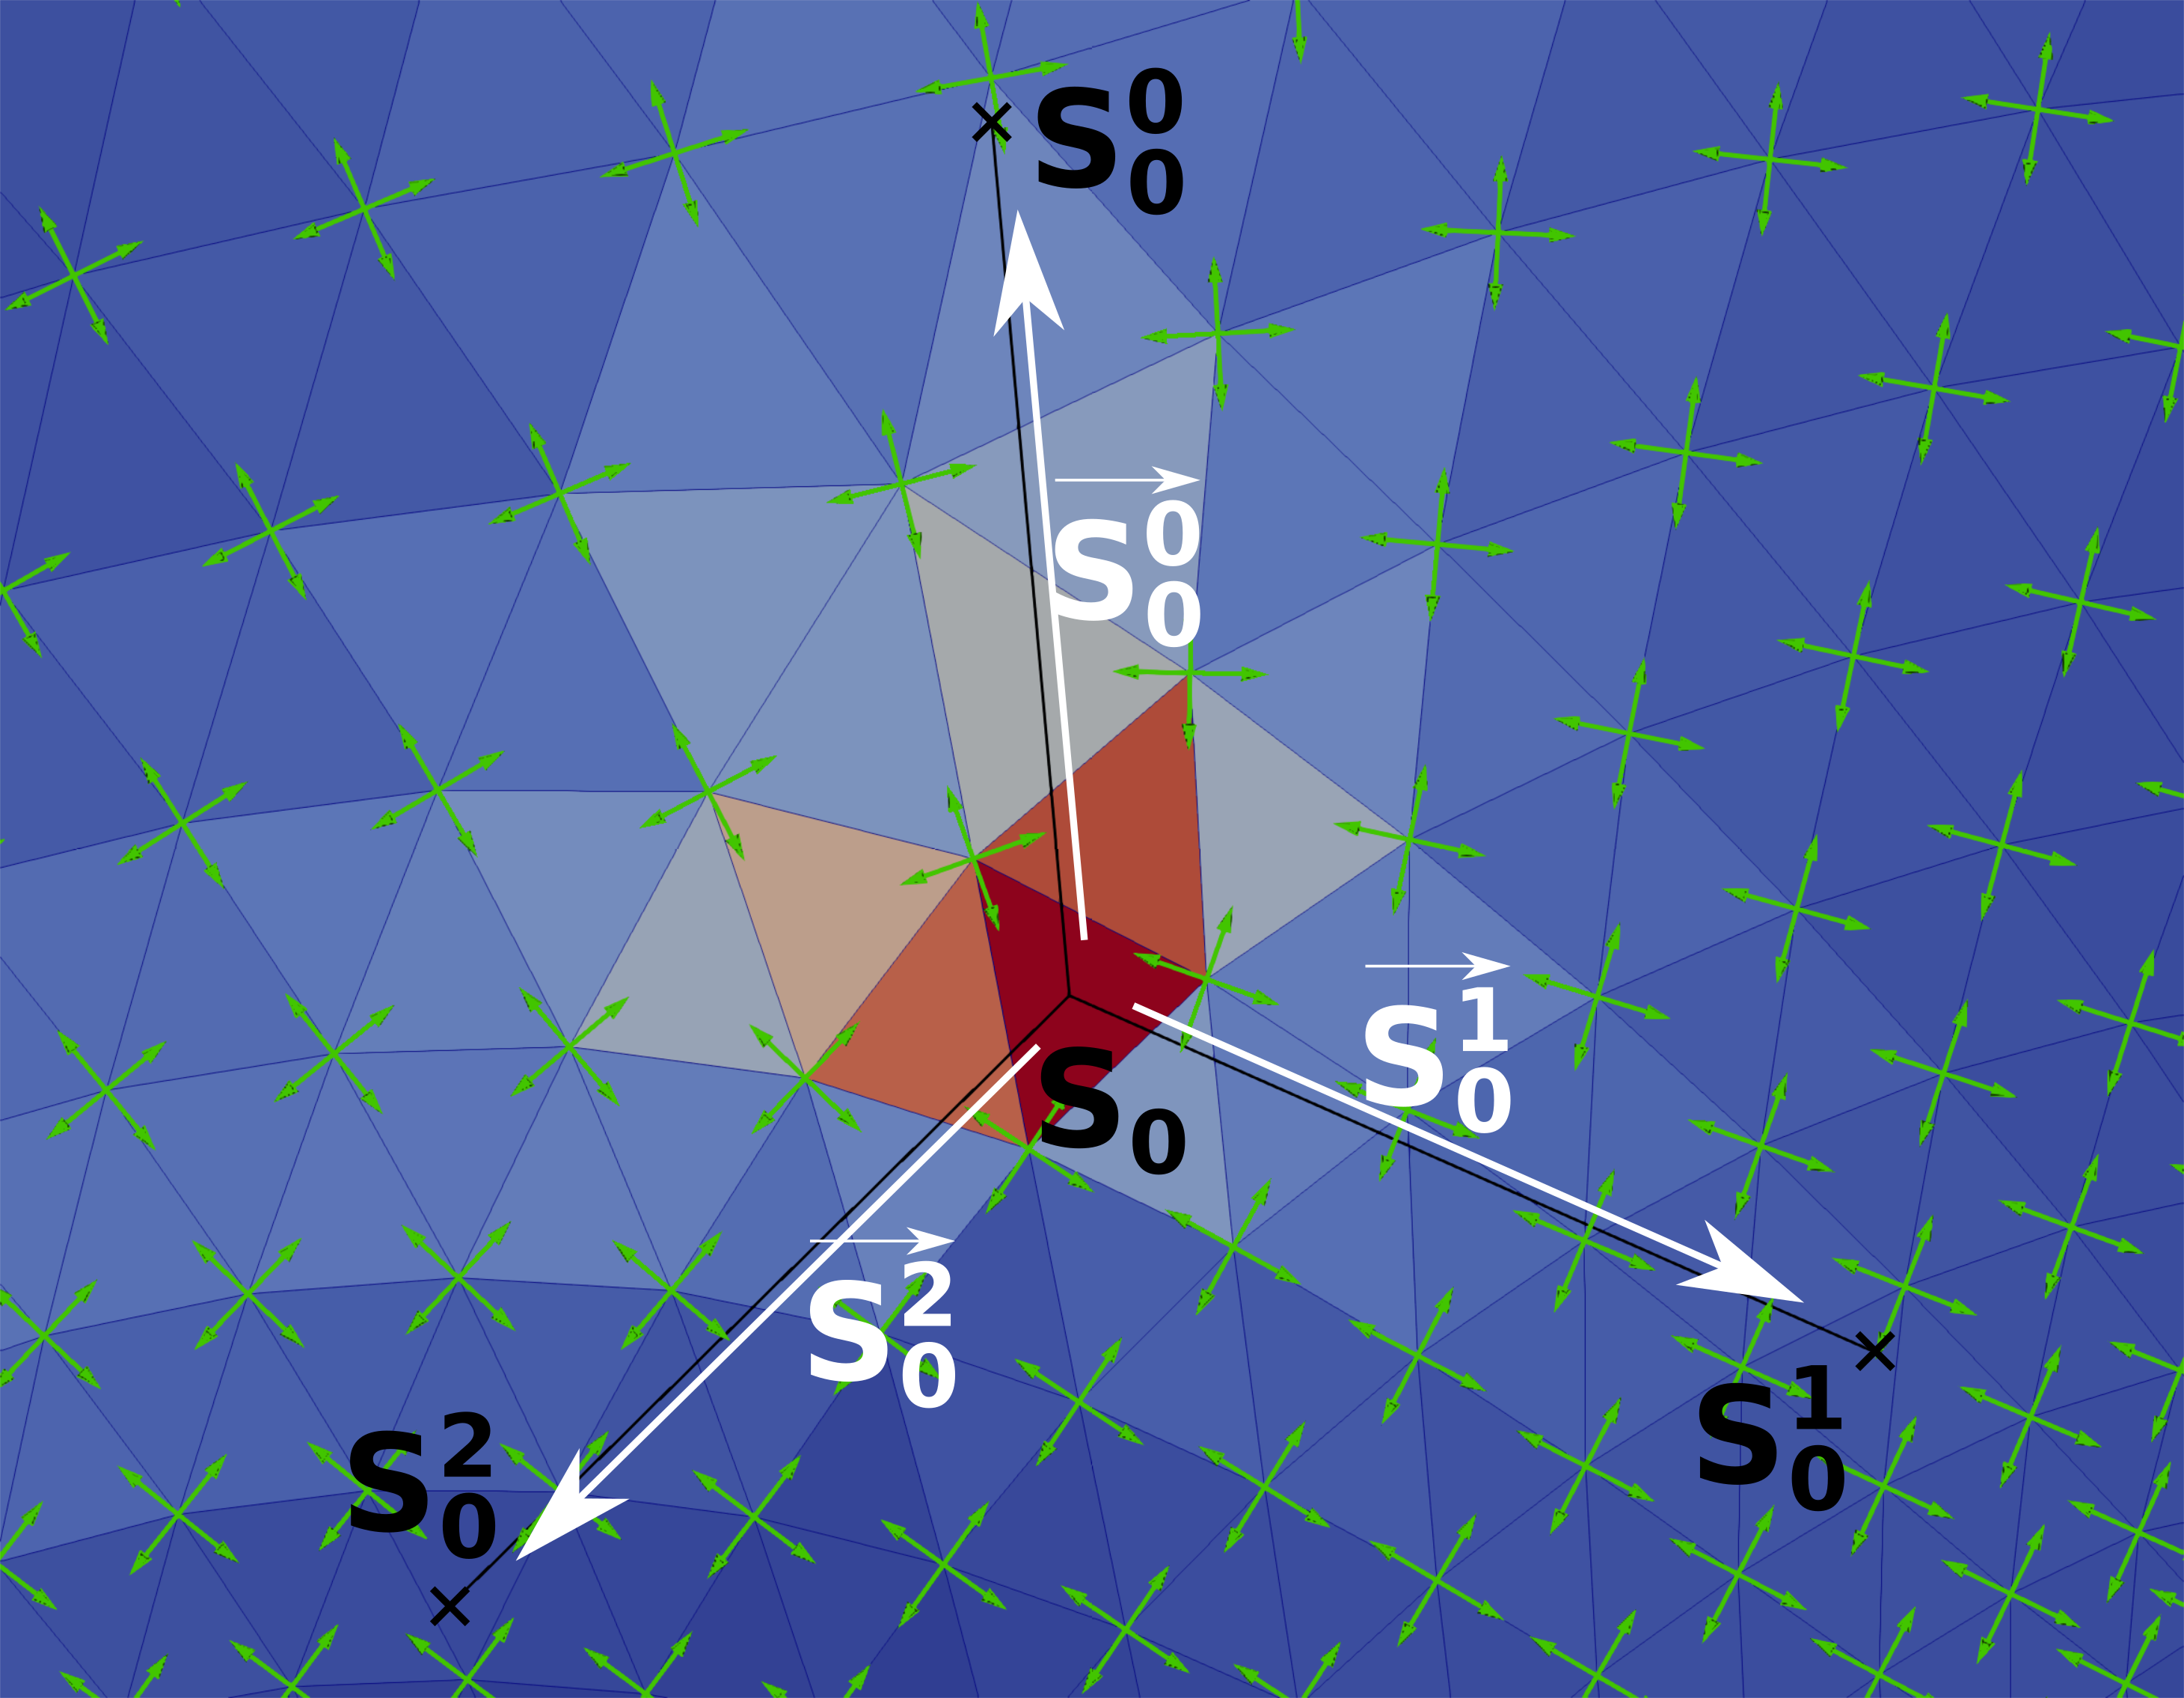
\includegraphics[width=0.95\textwidth]{SingSlots}
\caption{A 3-degree singularity and its slots}
\label{fig:singSlots}
\end{figure}

\medskip
 The first objective is to obtain a Shortest-Paths Graph $GSP \rightarrow (GSP_V, GSP_E)$, where the vertices are the total set of slot points plus the boundary ($GSP_V = S_{slots}^{points} \cup Bdry$) and the edges are the shortest paths between all possible pairs of slot points and the shortest paths all the slot points and the boundary ($GSP_E = SP[S_i^j; S_k^l] \cup SP[S_i^j; Bdry]; i,k=\overline{0,N}, j,l=\overline{0,4}$).

\bigskip

( \textcolor{blue}{createSingularityLinesShortestPaths()})
\newline
%\begin{equation}
% \underbrace{\bigintsss _{S} det(\textbf{J}) ds}_\text{area of the surface}  = \underbrace{\frac{1}{2} \bigintsss _{S} ||f_u||^2+ ||f_v^2||  ds}_\text{Dirichle's energy} - \underbrace{\frac{1}{2} \bigintsss _{S} ||f_v-rot_{90}(f_u X)||^2}_\text{conformal energy}
%\end{equation}


For each singularity point $S_i$ (situated inside a singular triangle) detect if at least one of its slots must be launched.
If so, for each such slot $S_i^j$, advance along the slots directions (using Runge-Kutta 4 - \textcolor{blue}{$growLineRK4()$}) until the landing faces are different.
\newline
If, during this procedure:
\newline
\begin{itemize}
\item we arrive at the boundary, we create and add this line to the final graph as a singularity line and we mark it as fixed for the optimization step (\textcolor{myGreen}{$addedAlready[i][j] =true;\newline possibleTargetTriangles[i][j] = original\_faces\_number + 1;$}). 
\item we arrive onto a slot of a different singularity that hasn't been connected, we create and add this line to the final graph as a singularity line and we mark it as fixed for the optimization step (\textcolor{myGreen}{$addedAlready[i][j] = true;$}). 

\end{itemize}

We will proceed now to the description of the two main steps of our algorithm:
\begin{itemize}
\item[•] The Shortest-Paths Step - current variable ID (streamline ID) will have the name \textcolor{myGreen}{$contSource$}.
\item[•] The Optimization Step - current variable ID (optimization matrix ID) will have the name \textcolor{myGreen}{$contMatrix$}.
\end{itemize}

\bigskip
\subsection{The Shortest-Paths Step}{
Our variables will be the slots of all the singularities (field singularities and geometric singularities, if the user has set \newline(\textcolor{myGreen}{$m\_build\_geometric\_singularities = true$})). We consider the total number of possible variables to be \textcolor{myGreen}{$totalNumberOfVariables$} $=$\textcolor{myGreen}{$totalNumberOfSlots$}$ + 1 = 5 * |S_{Pnts}| + 1 $; The $+ 1$ term arises because we also consider as variable the possible shortest path from a source slot towards the boundary, Fig.~\ref{fig:SPVar}. At each step of our algorithm the current variable ID (streamline ID) will have the name \textcolor{myGreen}{$contSource$}($ = 5*i+j;\ where\ i=\overline{0,|S_{Pnts}|}, j=\overline{0,4}$).
\begin{figure}[h]
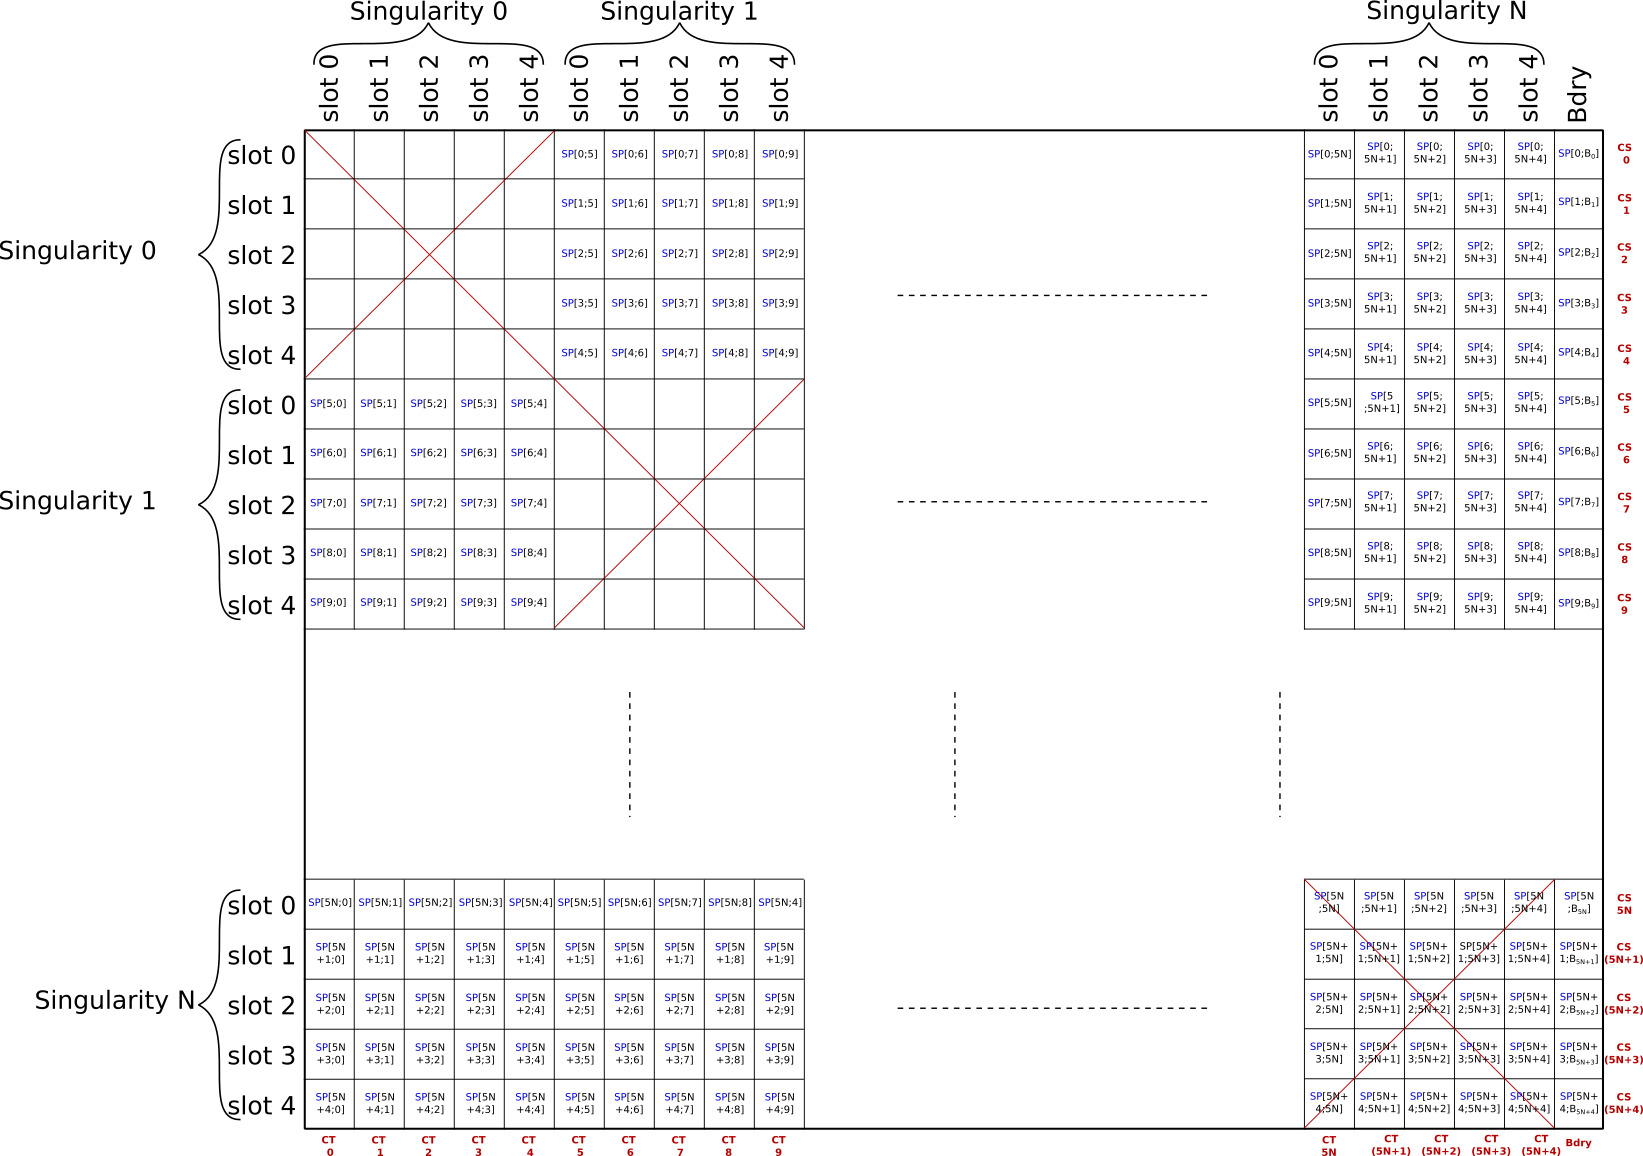
\includegraphics[width=0.95\textwidth]{ShortestPathsVariables}
\caption{Variables ilustrated as a matrix}
\label{fig:SPVar}
\end{figure}

Figures legend:
\begin{itemize}
\item[•] \textcolor{red}{$TNV$} $\leftarrow$ \textcolor{myGreen}{$totalNumberOfVariables$}
\item[•] \textcolor{red}{$TNS$} $\leftarrow$ \textcolor{myGreen}{$totalNumberOfSlots$}
\item[•] \textcolor{red}{$CS$} $\leftarrow$ \textcolor{myGreen}{$contSource$}
\item[•] \textcolor{red}{$CT$} $\leftarrow$ \textcolor{myGreen}{$contTarget$}
\item[•] \textcolor{red}{$SP$} $\leftarrow$ \textcolor{myGreen}{$Shortest Path$}
\end{itemize}



For each slot $S_i^j, i = \overline{0,N}, j = \overline{0,4}$ we store:
\begin{itemize}
\item $slot\_dir[contSource(=5*i+j)] = (-\overrightarrow{S_i^j }, -\overrightarrow{S_i^j })$
\end{itemize}

For each shortest path detected we must check whether it intersects a previous path detected and if so, the pair will be stored into \textcolor{myGreen}{$IllegalCross$}.
\begin{algorithmic}[1]
		\For{$i=\overline{0,N}$}
		\For{$j=\overline{0,4}$}
		\If{$addedAlready[i][j]==false$ and $\exists S_i^j$}
		\State $getShortestPaths(contSource, S_{slots}^{points} \cup Bdry)$
		
		\EndIf
		\EndFor
		\EndFor
		\end{algorithmic}	

\textcolor{blue}{$SingularityGraphBuilder2D::getShortestPathBtwFacesOptimized$}
		Get the shortest paths between the source slot \textcolor{myGreen}{$source$} and all other slots \textcolor{myGreen}{$targets$}.
		\newline
		Each of the \textcolor{myGreen}{$targets$} have associated the \textcolor{myGreen}{$targetPoints$} (the end points of their corresponding streamlines that have been propagated at the beginning) and the associated \textcolor{myGreen}{$slot\_dir$}. 
		\newline
		We increase the number of mesh triangles $|T|$ with the number of \textcolor{myGreen}{$targets$}, creating in this manner an artificial triangle ($T^{art}$) for each slot (\textcolor{myGreen}{$targets$} and the \textcolor{myGreen}{$source$}).
		\newline
		We define a vector of pairs \textcolor{myGreen}{$min\_distance$} which will store for each face:
		\begin{itemize} 
		\item  the "distance" that the path has travelled from the \textcolor{myGreen}{$source$} up until the current face  
		\item the number of visited triangles up until the current face.
		\end{itemize}		
		
		The distances for all the triangles will be initialized with the value 
		\textcolor{myGreen}{$maxDist$}$ = 10^6$
		
		Algorithm legend:
		\begin{itemize}
		\item $Q$ set of pairs $(dist[u], u)$, $ u \in M_T$
		\item $d = $ \textcolor{myGreen}{$min\_distance$}
		\item $T^{tot} = T + T^{art}$
		\item $N^{v}[u]$ - \textcolor{myGreen}{$face2Face\_neighbours\_by\_verts$}$[u]$
		\item $w\_{pen} = $\textcolor{myGreen}{$turnPenalizationTerm$} ($ = 0.1 * \textcolor{myGreen}{maxDist}$)
		\item $SD = slot\_dir$
		\item $CD = $ current direction (\textcolor{myGreen}{$tri2tri$})
		\item $T_c$ center point of triangle $T$
		\item $P^{art}$ - \textcolor{myGreen}{$targetPoints$} associated to the $T^{art}$
		\item $previous[u] = $ the triangle from which we have reached $u$ 
		\item $PDC[u]$ - previous direction cross of [u]
		\begin{itemize}
		\item $PDC[u].f$ - previous direction of triangle $u$ ($\overrightarrow{previous[u]_c, u_c} = CD$)
		\item $PDC[u].s$ - previous cross component vector of triangle $u$ (the cross component vector of $u$ that was the closest to the previous cross ($PDC[previous[u]].second$)) $ =  \widetilde{CT_u}$
		\end{itemize}
		 
		\item $\widetilde{CT_v}$ - the cross component vector of triangle $v$ that is the closest to  $PDC[u].second$
		\end{itemize}
		\begin{figure}[h]
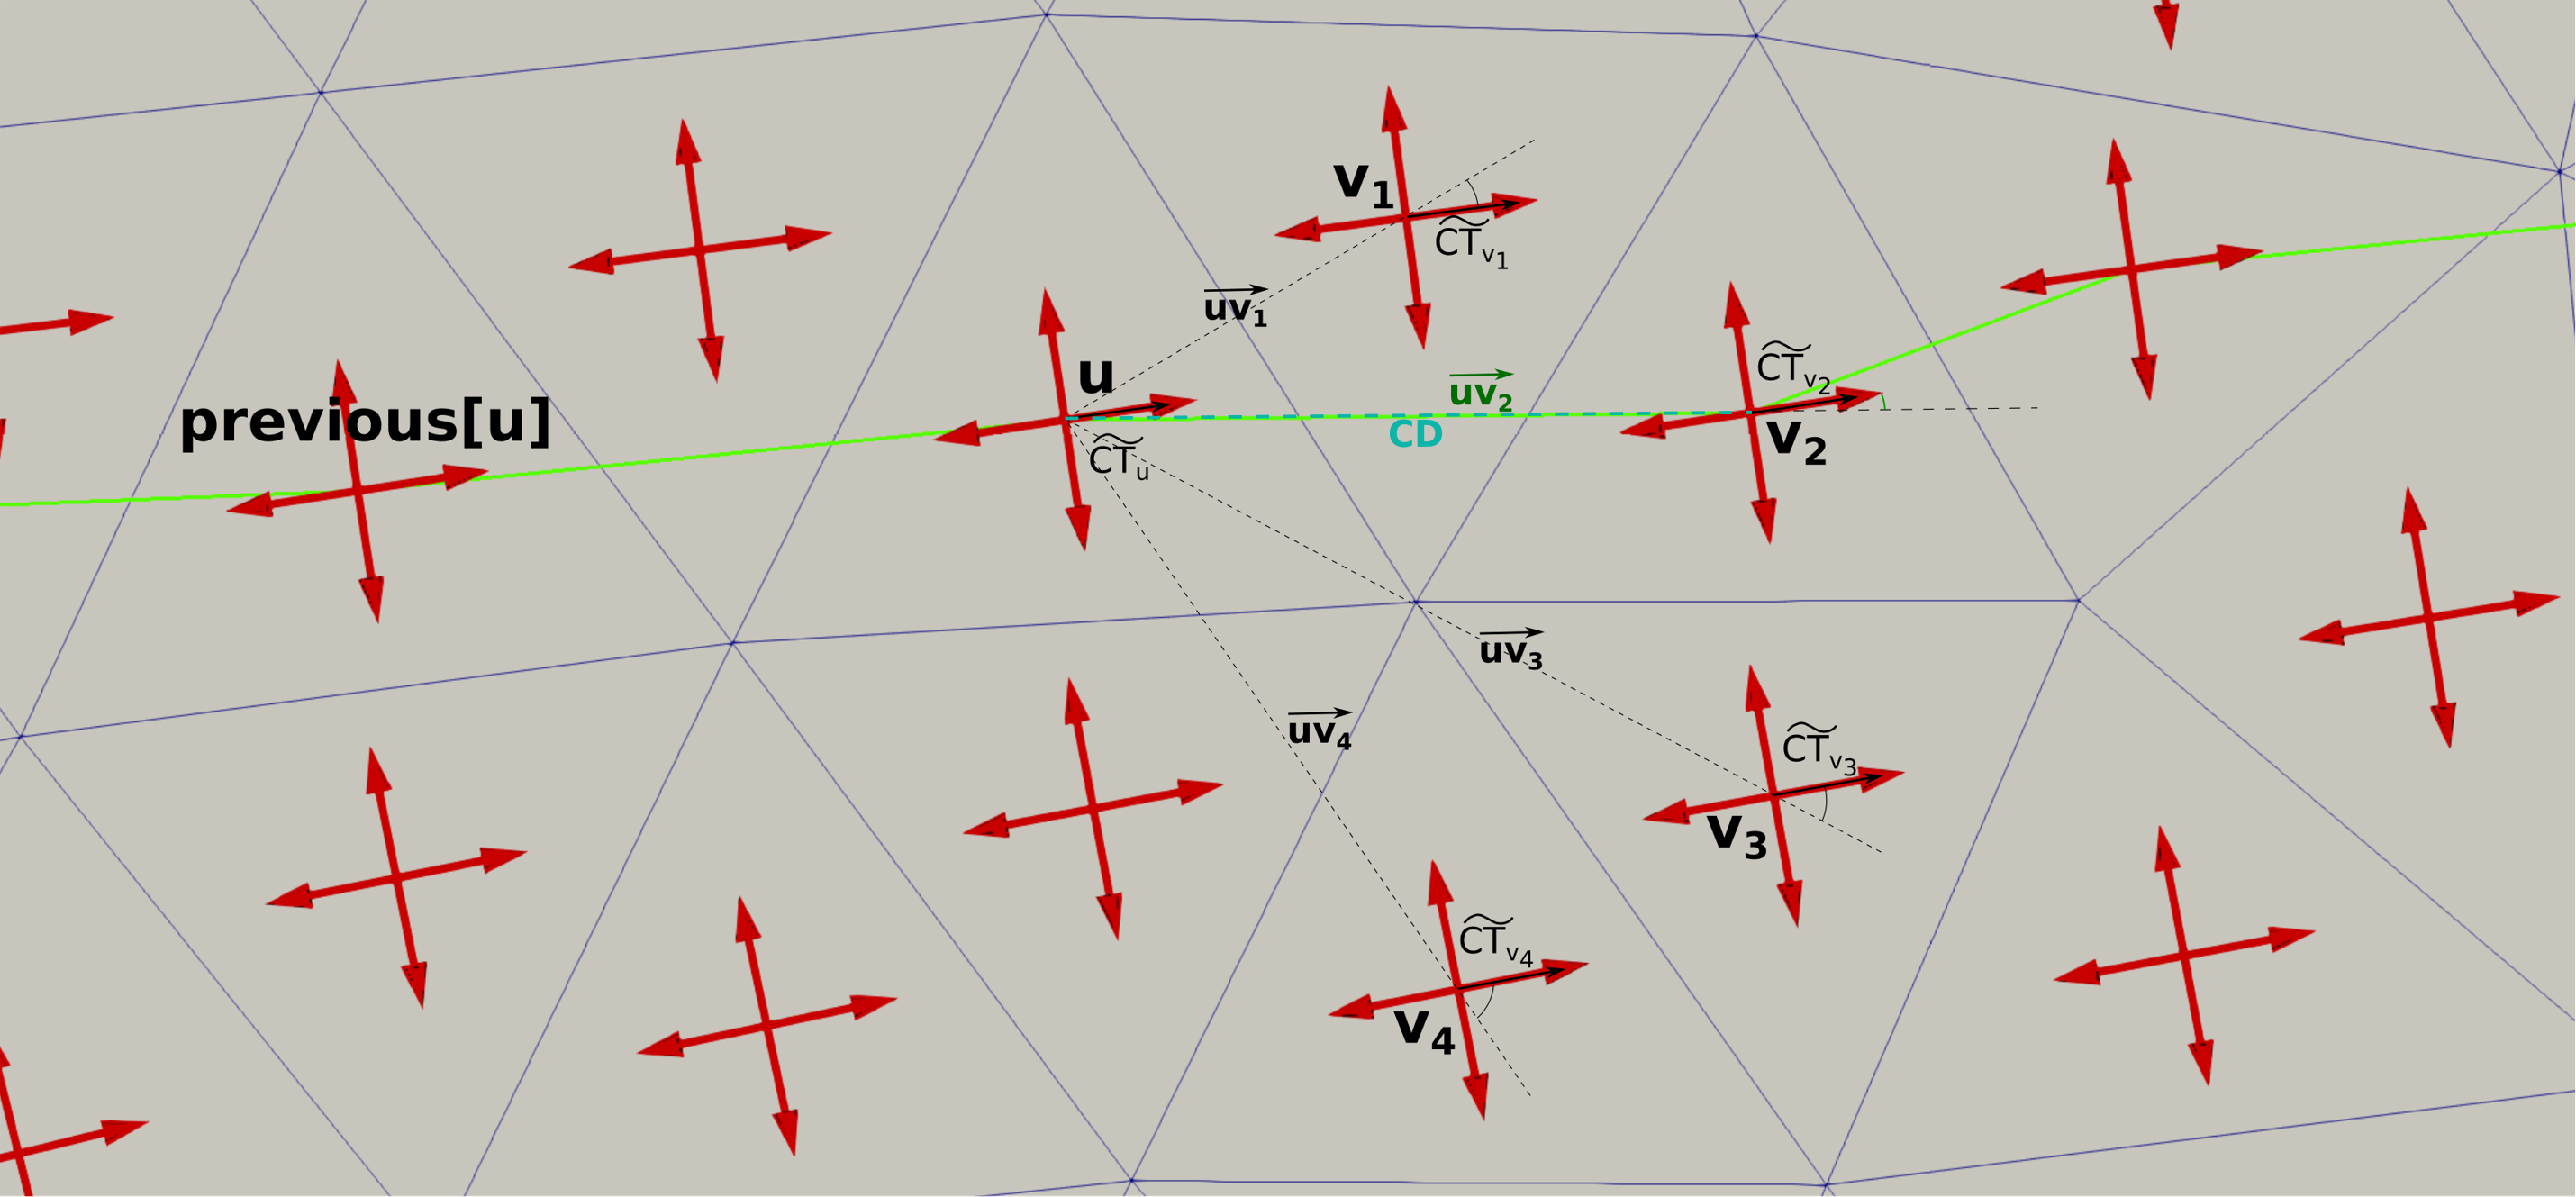
\includegraphics[width=0.5\textwidth]{shortestPaths-zoom2}
\caption{Shortest Paths Algorithm}
%\floatfoot{Completing a head: (a,d) the input mesh, (b,e) the template, (d,f) the completed model}
\end{figure}
\newpage
		\begin{algorithmic}[2]
		\For{$u\in M_T$}		
		\State $d[u] = maxDist (\infty)$
		\EndFor
		\State $d[source]\gets 0$
		\For{$u \in M_T$	}
		\State $Q \leftarrow (d[u], u)$
		\EndFor
		 
		%\State $d[T_{tot}]\gets maxDist$
		
		\While{$Q\not=\emptyset$}
		\State $u:= triangle\ in\ Q$
		%\State $d_{temp} = d[u]$	
		\State $Q\gets Q\setminus u$
			
		\If{$u\in N^{v}[T^{art}[i]]$}
		\State{$CD = \overrightarrow{u_c, P^{art}[i]}$}
		\State{$d_{temp} = d[u] + \angle(CD, PDC[u].s) + \angle(SD[T^{art}[i]], PDC[u].s) $}		
		\If{$ \angle(SD[T^{art}[i]], PDC[u].s)>\pi/4 || \angle(CD, PDC[u].s)>\pi/4 $}
		\State{$d_{temp} = d_{temp} + 3 * P$}		
		\EndIf
		\If{$d_{temp} < d[T^{art}[i]]$}
		\State $d[T^{art}[i]]\gets d_{temp}$		
		\EndIf
		\EndIf
		
		\If{$u\ -\ is\ boundary$}
		\State{$Ba = (1 - |dot(\angle(PDC[u].s), bdry\_normal))|)$}
		\footnote{$PDC[u].s$ and $bdry\_normal$ are normalized. Ideally, $|dot(\angle(PDC[u].s), bdry\_normal))| = 1$ (collinear) and in worst case scenario $|dot(\angle(PDC[u].s), bdry\_normal))| = 0$  (perpendicular), therefore we cannot connect to the boundary}
		\If{$ Ba<\pi/4$}
		\State{$d[bdry] = d[u] + Ba$}
		\EndIf
		\EndIf
		\For{$v\in Neigh(u); v\ not\ visited$}
		\State $CD = \overrightarrow{u_c, v_c}$
		\State $\widetilde{CT_v}\gets closest\ {CT_v}\ w.r.t\ PDC[u].s$
		\State $d_{temp} = d[u]+\angle(PDC[u].s,CD) + \angle(PDC[u].s,\widetilde{CT_v}) $
		\If($\angle(PDC[u].s,CD)>\pi/4$)
		\State $d_{temp} = d_{temp} + w\_{pen}$
		\EndIf
		
		\If{$d_{temp} < d[v]$}
		\State $d[v]\gets d_{temp}$
		\State $previous[v] = u$
		\State $PDC[v].s = \widetilde{CT_v}$
		\State $PDC[v].f = CD$
		\EndIf
		\EndFor
		\EndWhile
		\end{algorithmic}
		
		
		\newpage
		
		
		In the case of very coarse meshes which also have pairs of singularities that are close to one another (and at least one similar slot direction), it can happen that two possible streamlines converge Fig.~\ref{fig:ex2}.	
		If this situation arises, the user can set the variable \textcolor{myGreen}{$fixSPBdry = true;$}. In this case we will detect all pairs of \textcolor{myGreen}{$IllegalCross$} with both streamlines as boundary streamlines. We will recompute the higher-deviation streamline using only Runge-Kutta 4 and if it still intersects in an illegal manner its pair, we will also recompute the lower-deviation streamline. The result can be seen in Fig.~\ref{fig:ex3}.

\begin{figure}[h]
\includegraphics[width=0.95\textwidth]{Tomo_12000000_0000000_8000000_16_Rectangular_geo_ref1_want_graph}
\caption{Converging streamlines}
\label{fig:ex2}
%\floatfoot{Smt}
\end{figure}

\begin{figure}[h]
\includegraphics[width=0.95\textwidth]{Tomo_12000000_0000000_8000000_16_Rectangular_geo_ref1_correct_graph}
\caption{Recomputation of converging streamlines}
\label{fig:ex3}
%\floatfoot{Smt}
\end{figure}

\bigskip
\textcolor{blue}{$SingularityGraphBuilder2D::getTraversedTrisFaceNeighbyVertsExhaustive()$}
		After each possible streamline detection we apply this procedure. Since in our "Shortest Paths" algorithm we propagate from a face to one of its neighbouring faces by vertex, we will have a path consisting of triangles that are not necessarily adjacent by edge. This function detects the entire set of visited triangles. 
		Also, for each visited triangle this function will detect the direction of the possible streamline; for a triangle $u$, if the current \textbf{segment} ($CD$) is aligned to the $1^{st}$ or the $3^{rd}$ component vector of the cross field at the center of the triangle, we will insert the streamline ID into \textcolor{myGreen}{$isTraversedFaceCompVector[u].first$}$ \leftarrow contMatrix$. Otherwise (aligned to the $2^{nd}$ or the $4^{th}$ component vector), we insert the variable ID into \textcolor{myGreen}{$isTraversedFaceCompVector[u].second$}$ \leftarrow contMatrix$.
		
		At each such step we check whether the face has been traversed previously by a different possible streamline (\textcolor{myGreen}{$isTraversedFaceCompVector[u].x\ is\ not\  empty$}). If so, we detect if the segment (of that (or those) other streamlines that traverse the face with the same direction) intersects our current segment. If so, the pair of streamline ID's will be added to \textcolor{myGreen}{$IllegalCross$}.
		
		Since our streamline is not entirely made up of triangle centers, but rather source \textcolor{myGreen}{$line\_discretization$} $+$, triangle centers (\textcolor{myGreen}{$finalPaths$}) and possible $+$ target \textcolor{myGreen}{$line\_discretization$} (if streamline between 2 slots), we will also store a code (\textcolor{myGreen}{$isTraversedFaceCompVector\_SegmentPathCode[u].x$}) and a number indicating the position of segment (\textcolor{myGreen}{$isTraversedFaceCompVector\_SegmentPathCont[u].x$}); The codes are:
		\begin{itemize}
		\item[0] $\rightarrow$ the segment in the current face has both points in source \textcolor{myGreen}{$line\_discretization$}. If the segment is $[$\textcolor{myGreen}{$line\_discretization[contSource][i]$} , \textcolor{myGreen}{$line\_discretization[contSource][i+1]$} $]$, then \textcolor{myGreen}{$isTraversedFaceCompVector\_SegmentPathCont[u].x$ $\leftarrow i$}.
		\item[1] $\rightarrow$ the segment has 1 point in source \textcolor{myGreen}{$line\_discretization$} and the second point is the first triangle center of the Shortest Path ($[$\textcolor{myGreen}{$line\_discretization[contSource].back()$} , \textcolor{myGreen}{$finalPaths[contSource][0]$} $]$).
		\item[2] $\rightarrow$ the segment in the current face has both points as triangle centers. ($[$\textcolor{myGreen}{$finalPaths[contSource].[i]$} , \textcolor{myGreen}{$finalPaths[contSource][i+1]$} $]$).
		\item[3] $\rightarrow$ the segment has 1 point  as triangle center and the second point is the first (last actually, but it has been inversed) point of target \textcolor{myGreen}{$line\_discretization$} ($[$ \textcolor{myGreen}{$finalPaths[contSource].back()$} , \textcolor{myGreen}{$line\_discretization[contTarget][0]$}  $]$).
		\item[4]$\rightarrow$ the segment in the current face has both points in target \textcolor{myGreen}{$line\_discretization$}. ($[$\textcolor{myGreen}{$line\_discretization[contTarget].[i]$} , \textcolor{myGreen}{$line\_discretization[contTarget][i+1]$} $]$).
		\item[5] $\rightarrow$ the segment has 1 point  as triangle center and the second point is the boundary intersection point \textcolor{myGreen}{$finalEndPoint$} ($[$ \textcolor{myGreen}{$finalPaths[contSource].back()$} , \textcolor{myGreen}{$finalEndPoint[contSource]$}  $]$).
		\end{itemize}
 
			
		
		
		
}

\newpage
\subsection{The Optimization Step}{

Now we want to detect the final graph $G \rightarrow (V, E)$, where $V = S_i^j \cup B_x;  i = \overline{0,N} , j = \overline{0,4} , B_x -$the end points of the boundary streamlines that have been detected as belonging to the final graph and $E = SP^*[a;b]$ - the optimal set of shortest paths between pairs of slots/boundary ($a,b$).

Our variables will be $x[i] = {0,1}$ - corresponding to the presence or absence of all the possible shortest paths, therefore a total number of \textcolor{myGreen}{$totalNumberOfSlots$} $ * $ \textcolor{myGreen}{$totalNumberOfVariables$}, where 
 \textcolor{myGreen}{$totalNumberOfVariables$} $=$ \textcolor{myGreen}{$totalNumberOfSlots$} $+1$. At each step of our algorithm the current optimization variable ID will have the name \textcolor{myGreen}{$contMatrix$}($ = contSource*totalNumberOfVariables + t;$ where $t=\overline{0,|contSource|+1}$).

After our previous step we have the entire set of possible shortest paths, as well as their weights (deviations from the field) $d$, Fig.~\ref{fig:optVar}. 

\begin{figure}[h]
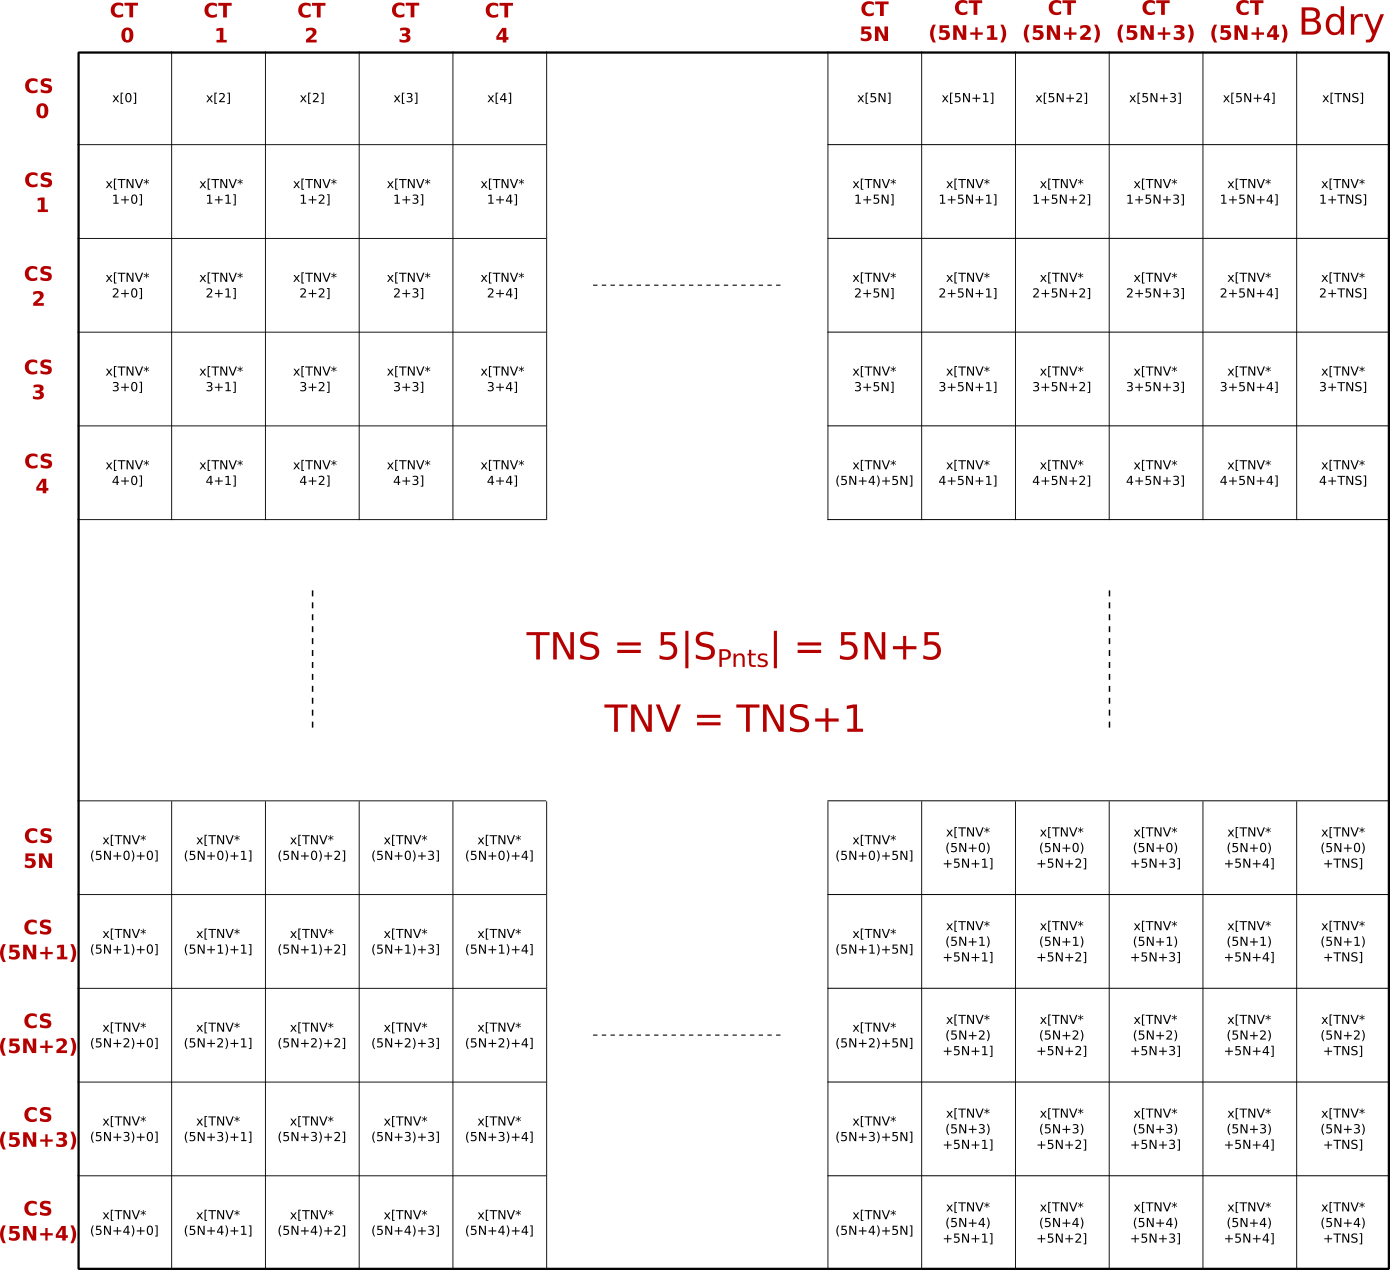
\includegraphics[width=0.95\textwidth]{optVar}
\caption{Optimization variables - General Setup}
\label{fig:optVar}
\end{figure}

\begin{figure}[h]
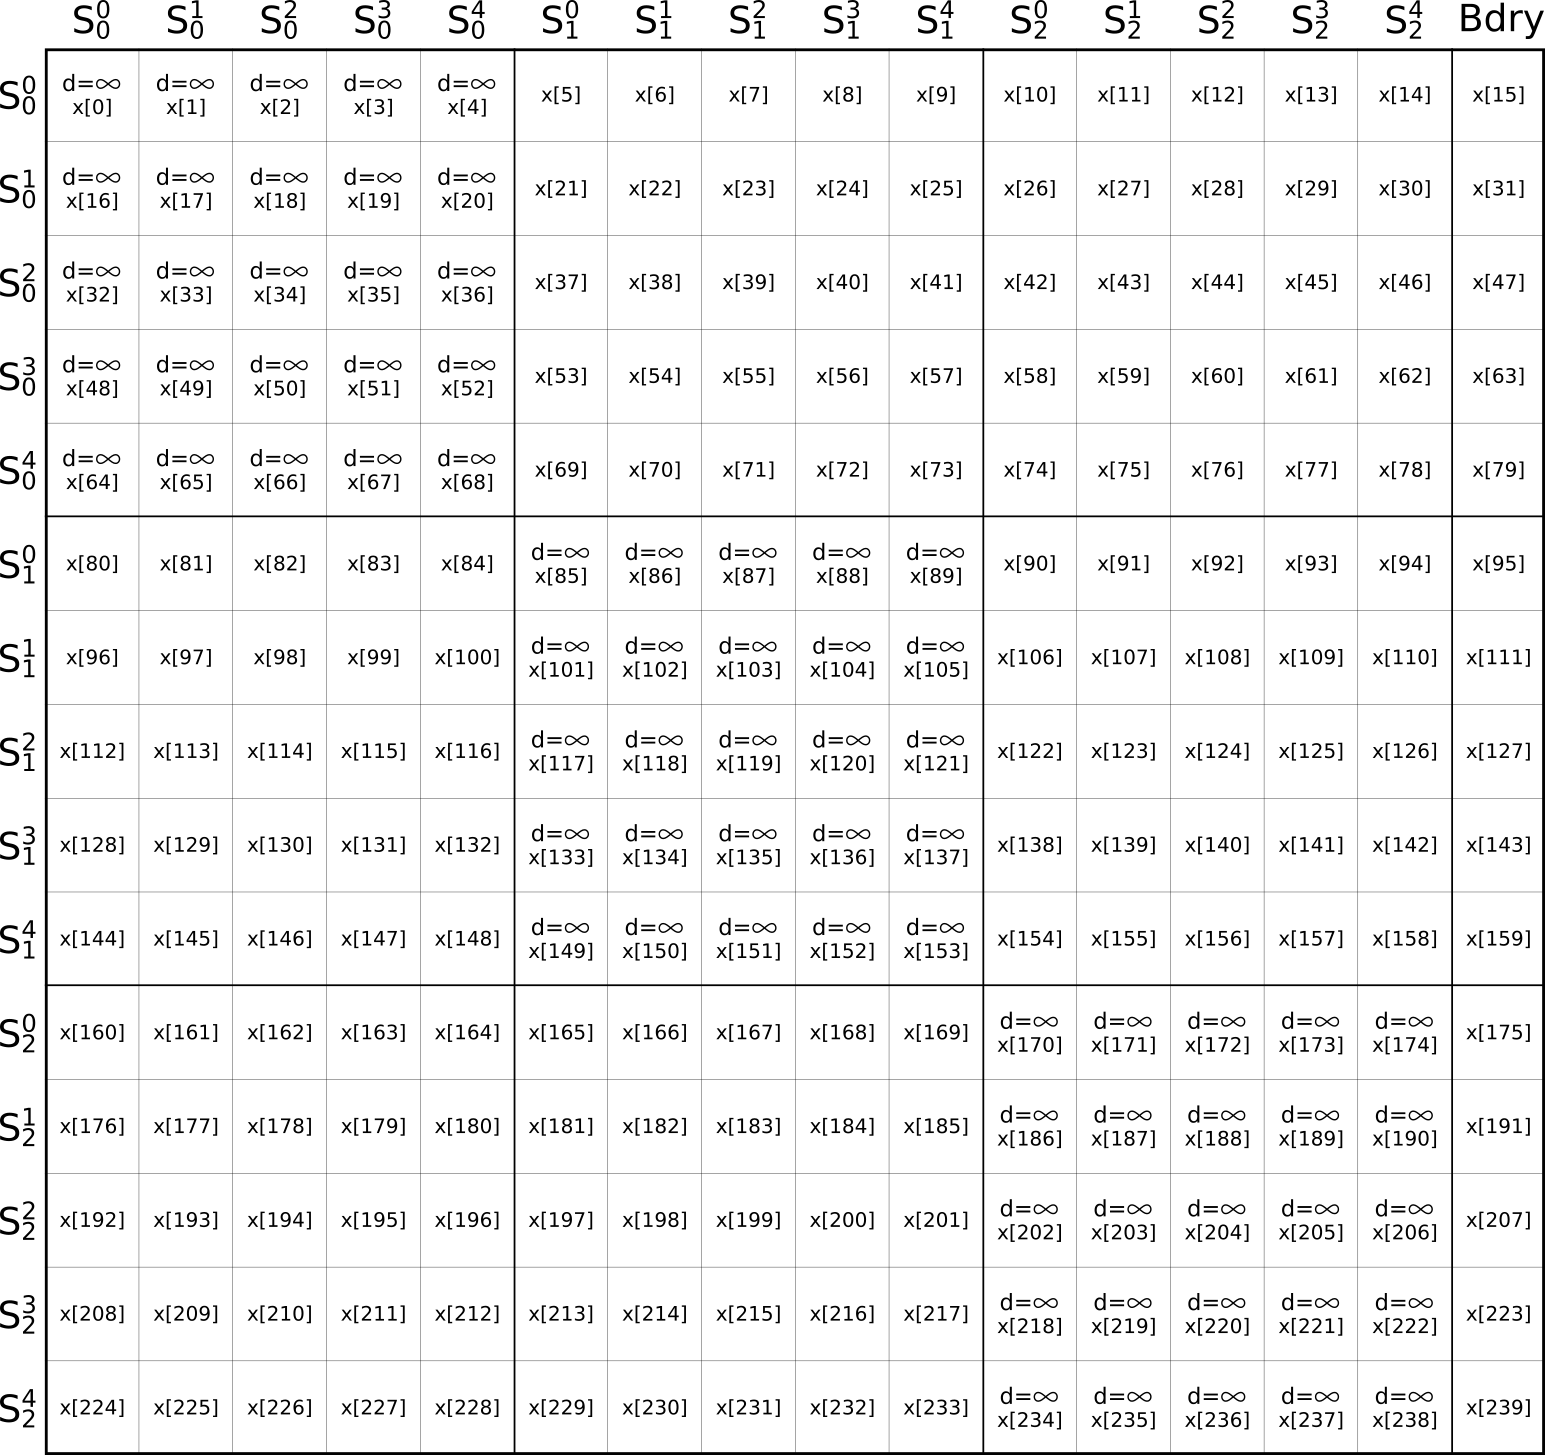
\includegraphics[width=0.95\textwidth]{optVarEx}
\caption{Optimization variables - Example 3 singularity points}
\label{fig:optVarEx}
\end{figure}

	If we denote our variables as $x[t]$ and their weights as $d[t]$, 
	where $t = CS * TNV + CT$, the system that we must solve in order to obtain the final graph is: 
	\newline
	$$ min \left(\sum_{i=0}^{TNV*TNS} (x[i]*d[i])\right) , x[i] \in {0,1}$$

	respecting the following conditions:
	\begin{itemize}
	\item[a)] From each slot exactly one path must be kept.
		$\sum_{j=0}^{TNS+1} (x[i*TNS+j]) + \sum_{k=0}^{TNS} (x[k*TNS+i]) = 1,  \forall i = \overline{0,TNS-1}$
	\newline
	$(SP[i,:] + SP[:i] \leq 1, \forall i = \overline{0,TNS-1})$
	
	\item[b)] A maximum of one path must be kept from each pair of incompatible paths \textcolor{myGreen}{$IllegalCross$}.  
	$ \forall (x[a], x[b]) \in IllegalCroos, x[a] + x[b] \leq 1$.
	\item[c)] A slot is allowed to connect only with slots belonging to other singularities. (This condition can be removed).
	$ x[a] = x[b] = 0, if a\%5 = b\%5 $.	

	\end{itemize}
	

	

%Fig.~\ref{fig:SPVar}
}

































\begin{comment}

\begin{figure}[H]

\includegraphics[width=0.5\textwidth]{img/mesh_completion.png}
\caption{Mesh Completion \cite{KraevoyS05}}
\floatfoot{Completing a head: (a,d) the input mesh, (b,e) the template, (d,f) the completed model}
\end{figure}

\begin{figure}[H]
\includegraphics[width=0.9\textwidth]{img/remesh-cpcr.png}
\caption{Remeshing \cite{Kraevoy2004}}
\floatfoot{a) source mesh, b) target mesh after initial projection, c) smoothing step, d) final mesh}
\end{figure}
\end{comment}
}
\newpage
\subsection{Subsection}

{ Subsection
\begin{comment}
\begin{equation}
\begin{split}
 \frac{\partial v}{\partial x}  =  -\frac{\partial u}{\partial y} \\
 \frac{\partial v}{\partial y}  =   \ \ \frac{\partial u}{\partial x}
 \end{split}
\end{equation}



\begin{equation}
\sum\nolimits_{v_i \in M \setminus \partial M} K_i + \sum\nolimits_{v_i \in \partial M} k_i = 2 \pi \chi(M)
\end{equation}
where
\begin{equation}
\chi(M)=|T|-|E|+|V|
\end{equation}
\end{comment}

}

\subsubsection{Subsubsection}

{Subsubsection
\begin{comment}
\begin{figure}[H]
\subcapcentertrue
   \subfigure[MIPS \cite{Hormann2000}]{\includegraphics[scale=0.4]{img/mips.png}}
 \subfigure[ABF++ \cite{Sheffer2005}]{\includegraphics[scale=0.4]{img/ABFplus.png}}
  \subfigure[Circle patterns \cite{Kharevych06}]{\includegraphics[scale=0.4]{img/circle.png}}
\caption{Nonlinear conformal maps  \cite{Hormann2007}}
 \end{figure}

\begin{figure}[H]
\includegraphics[width=0.5\textwidth]{img/kharevych.png}
\caption{Circle patterns \cite{Kharevych06}}
\floatfoot{Comparison of 2 mappings of the Lion data set: natural boundaries and disk boundary. Error plots - quasiconformal distortion between original and mapped triangles\protect\footnotemark}
\end{figure}
\footnotetext{quasiconformal distortion = ratio between the largest and smallest eigenvalue of the Jacobian matrix of the mapping; ideal=1}
\end{comment}

}
\subsubsection{Subsubsection}

{ Subsubsection

%\footnotetext{quasiconformal distortion = ratio between the largest and smallest eigenvalue of the Jacobian matrix of the mapping; ideal=1}

% \footnotetext{desired angle sum of $ \pi $ at all vertices, except four (the corners of the rectangle), for which the desired angle sum is $ \pi/2 $.}

}
\newpage
\subsection{Subsection}

{ Subsection



}
\begin{comment}

\newpage
\subsection{Table results Ex}

{

    \hskip-3.5cm\begin{tabular}{ | p{2cm} || p{2cm} | p{2cm} | p{2cm} | p{2cm} | p{2cm} | p{2cm} |p{2cm} |}
    \hline
   

 Method                     &\multicolumn{1}{|c|}{\textbf{CFCPMS}}                                                                                       &\multicolumn{1}{|c|}{\textbf{CETM}}    &\multicolumn{1}{|c|}{\textbf{MAAM}}                &\multicolumn{1}{|c|}{\textbf{MVC}}                                                                             &\multicolumn{1}{|c|}{\textbf{LSCM}}  &\multicolumn{1}{|c|}{\textbf{DCP}}                                            & \multicolumn{1}{|c|}{\textbf{ABF/ABF++}}              \\
                            &\multicolumn{1}{|c|}{\textbf{2008}}                                                                                         &\multicolumn{1}{|c|}{\textbf{2008}}    &\multicolumn{1}{|c|}{\textbf{1995}}                &\multicolumn{1}{|c|}{\textbf{2003}}                                                                            &\multicolumn{1}{|c|}{\textbf{2002}}  &\multicolumn{1}{|c|}{\textbf{2002}}                                           & \multicolumn{1}{|c|}{\textbf{2000/2005}}              \\ \hline
 Parameter Domain           & plane                                                                                                                      &plane and sphere                       &    plane                                          & plane                                                                                                         & plane                         & plane                                                                              & plane                                                \\ \hline
 Automatic                  & yes                                                                                                                        &yes (optionally user intervention)     &  yes                                              &  yes                                                                                                          &  yes                          &yes (optionally user intervention)                                                  & yes                                                  \\ \hline
 Minimized distortion       &angle (but in practice area also)                                                                                           &angle                                  &angle                                              &angle                                                                                                          &angle(and area)                & angle(and area)                                                                    & angle                                                \\ \hline
 Boundary                   &free                                                                                                                        & fixed/free                            &fixed, convex                                      &fixed, convex                                                                                                  &free                           &free/fixed                                                                          &free                                                  \\ \hline
 Topology                   &Arbitrary With or without boundary                                                                                          &Arbitrary With or without boundary     &Arbitrary                                          & -                                                                                                             & -                             &Arbitrary (Non-closed surfaces)                                                     & Arbitrary                                            \\ \hline
 Input mesh                 &2-142K                                                                                                                      & H-209K                                & 100K $\Delta$                                     & 257$\Delta$-78K$\Delta$                                                                                       &14.5K - 48.5K                  & 257$\Delta$-78K$\Delta$                                                            & 68-879$\Delta$                                       \\ \hline
 Number of feature vertices &12-106                                                                                                                      & 4-18                                  & -                                                 & -                                                                                                             & -                             & -                                                                                  & -                                                    \\ \hline
 Code available             &   yes                                                                                                                      &no                                     &no                                                 &no                                                                                                             &yes                            &no                                                                                  &no                                                    \\ \hline
 Bijectivity                & no                                                                                                                         & no                                    &no(yes-only if mesh satisfies Delaunay criterion)  &yes                                                                                                            & no                            & no                                                                                 &locally(no flips),but can contain global overlaps    \\ \hline   
 Optimization System        &linear                                                                                                                      & non-linear                            &linear                                             &linear                                                                                                         &linear                         &linear                                                                              &non-linear                                            \\ \hline                                                                       
 %Numerical solution
 Timing / Complexity        &Fast                                                                                                                        & 162s$\rightarrow$209K                 & 0.02s$\rightarrow$257$\Delta$                     &0.02s$\rightarrow$257$\Delta$                                                                                  &0.03s$\rightarrow$257$\Delta$  &5s-fixed boundary                                                                   &0.06s$\rightarrow$257$\Delta$                        \\
                            &\multirow{4}{*}{\parbox{2cm}{boundary increases $\Rightarrow$ time increases}}                                              & 230s$\rightarrow$142K                 & 0.17s$\rightarrow$6K$\Delta$                      &0.16s$\rightarrow$6K$\Delta$                                                                                   &0.2s$\rightarrow$6K$\Delta$    &\multirow{3}{*}{\parbox{2cm}{15s-optimized boundary}}                               & 0.77s$\rightarrow$6K$\Delta$                         \\  
                            &                                                                                                                            & (more iterations)                     & 0.26s$\rightarrow$8K$\Delta$                      &0.25s$\rightarrow$8K$\Delta$                                                                                   &0.38s$\rightarrow$8K$\Delta$   &                                                                                    &1.87s$\rightarrow$8K$\Delta$                          \\
                            &                                                                                                                            &                                       & 3.21s$\rightarrow$78K$\Delta$                     &3.19s$\rightarrow$78K$\Delta$                                                                                  &5.28s$\rightarrow$78K$\Delta$  &                                                                                    &36.31s$\rightarrow$78K$\Delta$                        \\
                            &                                                                                                                            & 1.1GHz Pentium M                      & 346.6s$\rightarrow$166K $\Delta$                  &                                                                                                               &                               &                                                                                    &                                                      \\ \hline                                                                        
 Observations               &Simple to implement                                                                                                         & \multirow{6}{*}{\parbox{2cm}{Overall distortion worse than CFCPMS}}  &\multirow{9}{*}{\parbox{2cm}{Simple to implement}} &Simple to implement                                                                                            &\multirow{6}{*}{\parbox{2cm}{No overlapping triangles}}       &\multirow{6}{*}{\parbox{2cm}{Visible discontinuities along cuts}}      &\multirow{9}{*}{\parbox{2cm}{Significantly less stretch for models with high Gaussian curvature}}      \\                                                                                                                                                                                                                                                    
                            &Seamless metrics not considered                                                                                             &                                       &                                                   & \multirow{7}{*}{\parbox{2cm}{In some cases may introduce larger angular distortion than harmonic weights}}    &                               &                                                                                    &                                                       \\ \cline{6-7} \cline{2-3} 
                            & \multicolumn{2}{|c|}{\multirow{4}{*}{\parbox{4cm}{Main difference: algorithm to manipulate the curvature distribution }}}                                          &                                                   &                                                                                                               &\multicolumn{2}{|c|}{\multirow{3}{*}{\parbox{4cm}{Significantly less distortion than fixed boundary approaches}}}   &                                                      \\         % \rule{0cm}{2cm}     
                            &   \multicolumn{2}{|c|}{}                                                                                                                                           &                                                   &                                                                                                               &\multicolumn{2}{|c|}{}                                                                                              &                                                      \\                                                                                                                                                                                                                               
                            &    \multicolumn{2}{|c|}{}                                                                                                                                          &                                                   &                                                                                                               & \multicolumn{2}{|c|}{}                                                                                             &                                                       \\                                                                                                                            
                            &     \multicolumn{2}{|c|}{}                                                                                                                                         &                                                   &                                                                                                               & \multicolumn{2}{|c|}{}                                                                                             &                                                       \\ \hline                                                                                                                           
 \end{tabular}

}




 \newpage
\subsection{SubSection5}
{SubSection

}
 \newpage
\subsection{Table Res}

{
\setlength\LTleft{-1in}
\setlength\LTright{-1in}
   \hskip-5cm\begin{longtable}[0.5]{ | p{2.5cm} || p{2.5cm} | p{2.5cm} | p{2.5cm} | p{2.5cm} | p{2.5cm} |}
    \hline

 Method                     & \multicolumn{1}{|c|}{\textbf{CPCR}}                                                                                        &  \multicolumn{1}{|c|}{\textbf{ISM}}                                              & \multicolumn{1}{|c|}{\textbf{LBLDSM} }            &\multicolumn{1}{|c|}{\textbf{MVSC}}                                                                            & \multicolumn{1}{|c|}{\textbf{BIM}}                                     \\
                            & \multicolumn{1}{|c|}{\textbf{2004}}                                                                                        &   \multicolumn{1}{|c|}{\textbf{2004}}                                            &\multicolumn{1}{|c|}{\textbf{2014}}                & \multicolumn{1}{|c|}{\textbf{2009}}                                                                           & \multicolumn{1}{|c|}{\textbf{2011}}                                    \\ \hline
 Automatic                  & No                                                                                                                         &No                                                                                &  No                                               & yes                                                                                                           & yes                                                                     \\ \hline
 Minimized distortion       & shape                                                                                                                      &scale                                                                             &                                                   & - (length / area)                                                                                             & angle / area                                                            \\ \hline
 Boundary                   &                                                                                                                            &                                                                                  &                                                   &                                                                                                               &                                                                         \\ \hline
 Remeshing / Mapping Based  &remeshing                                                                                                                   & remeshing                                                                        &                                                   & mapping based                                                                                                 &mapping based                                                            \\ \hline
 Topology                   &Arbitrary                                                                                                                   &Arbitrary                                                                         &                                                   & sphere                                                                                                        & genus 0                                                                 \\ 
                            &  (but only genus 0 guaranteed)                                                                                             & With or without boundary (with holes)                                            &                                                   & (with or without boundary, with holes)                                                                        &                                                                         \\ \hline                                                                                                   
 Input mesh                 &1.7K-39K                                                                                                                    & 2.9-64K                                                                          &                                                   & V=                                                                                                            &12-35K                                                                   \\ \hline
 Number of feature vertices &15-28                                                                                                                       & genus 0 $\geq$ 4                                                                 &                                                   &\multirow{3}{*}{\parbox{2.5cm}{(N=$\sim$100 random feature samples)}}                                          & 5 $\rightarrow$ 12.5K                                                   \\ 
                            & ($\geq$ 4 per handle)                                                                                                      & genus 1 $\rightarrow$ 22                                                         &                                                   &                                                                                                               & 6 $\rightarrow$ 27.9K                                                   \\                                                                                                                                                                                                                     
                            &                                                                                                                            &\multirow{1}{*}{\parbox{2.5cm}{genus 2 $\rightarrow$ 8 (user) + 7 (automatically)}}&                                                  &                                                                                                               & \multirow{1}{*}{\parbox{2.5cm}{($\sim$ 100 random feature samples)}}      \\                                                                                                                                     
                            &                                                                                                                            &                                                                                  &                                                   &                                                                                                               &                                                                         \\                                                       
                            &                                                                                                                            &                                                                                  &                                                   &                                                                                                               &                                                                         \\ \hline
 Code available             & no                                                                                                                         &no                                                                                &no                                                 &no                                                                                                             &yes                                                                      \\ \hline
 Bijectivity                & yes                                                                                                                        & yes                                                                              &yes                                                &no                                                                                                             & no                                                                      \\ \hline   
 Numerical Optimization     & ?                                                                                                                          &  non-linear                                                                      &  non-linear                                       &polynomial time                                                                                                & polynomial time                                                         \\ \hline                                                                 
 Timing / Complexity        & $\sim$120s $\rightarrow$ 10K                                                                                               & \multirow{5}{*}{\parbox{2.5cm}{hours for $\sim$64K}}                             &                                                   &$O(N^4\log N+V^2\log V)$                                                                                       & 80s $\rightarrow$ 12.5K                                                 \\                                                                        
                            & $\sim$120s $\rightarrow$ 64K                                                                                               &                                                                                  &                                                   & 70s $\rightarrow$ N=80                                                                                        & 384s $\rightarrow$ 27.9K                                                 \\                          
                            & 59s $\rightarrow$ 40K$\Delta$                                                                                              &                                                                                  &                                                   & 160s $\rightarrow$ N=120                                                                                      & worst: 2100s $\rightarrow$ 53K                                           \\                 
                            & 56s $\rightarrow$ 80K.7K$\Delta$                                                                                           &                                                                                  &                                                   & (1M votes)                                                                                                    & \multirow{3}{*}{\parbox{2.5cm}{Time depends on N and V}}                   \\                 
                            & (texture transfer)                                                                                                         & \multirow{2}{*}{\parbox{2.5cm}{High computational complexity}}                   &                                                   & \multirow{2}{*}{\parbox{2.5cm}{$\sim$6min $\rightarrow$ K meshes}}                                            &                                                                          \\                   
                            & \multirow{2}{*}{\parbox{2.5cm}{3GHz pentium IV}}                                                                           &                                                                                  &                                                   &                                                                                                               & \multirow{4}{*}{\parbox{2.5cm}{2.2GHz Opteron 275 processor}}              \\                                                                   
                            &                                                                                                                            &                                                                                  &                                                   & \multirow{3}{*}{\parbox{2.5cm}{2.2GHz Opteron 275 processor}}                                                 &                                                                          \\                                                                                                          
                            &  \multirow{2}{*}{\parbox{2.5cm}{Faster than ISM}}                                                                          & \multirow{2}{*}{\parbox{2.5cm}{extremely slow}}                                  &                                                   &                                                                                                               &                                                                          \\                                                                                             
                            &                                                                                                                            &                                                                                  &                                                   &                                                                                                               &                                                                          \\  \hline 
Overall Distortion          &  \multirow{4}{*}{\parbox{2.5cm}{$E_{ang}=[0.04, 0.18]$}}                                                                   & \multirow{8}{*}{\parbox{2.5cm}{$L2_{symm-stretch}=[0.598, 0.311]$}}              &                                                   &\multirow{4}{*}{\parbox{2.5cm}{45 corresp $\leq$ 3$\%$ error - same obj in diff poses}}                        &\multirow{4}{*}{\parbox{2.5cm}{$\epsilon=[0,0.66]$}}                        \\ 
                            &                                                                                                                            &                                                                                  &                                                   &                                                                                                               &                                                                          \\   
                            &                                                                                                                            &                                                                                  &                                                   &                                                                                                               &                                                                          \\  
                            &                                                                                                                            &                                                                                  &                                                   &                                                                                                               &                                                                          \\                             
                            & \multirow{4}{*}{\parbox{2.5cm}{$L2_{stretch}=[0.86, 0.05]$}}                                                               &                                                                                  &                                                   &\multirow{4}{*}{\parbox{2.5cm}{15 corresp $\leq$ 3$\%$ error - same person in diff poses - scan}}              &\multirow{4}{*}{\parbox{2.5cm}{$Max_\epsilon=1.37$}}                        \\   
                            &                                                                                                                            &                                                                                  &                                                   &                                                                                                               &                                                                          \\                              
                            &                                                                                                                            &                                                                                  &                                                   &                                                                                                               &                                                                          \\  
                            &                                                                                                                            &                                                                                  &                                                   &                                                                                                               &                                                                          \\   \hline 
 \pagebreak
 \hline
 Method                     &  \multicolumn{1}{|c|}{\textbf{CPCR}}                                                                                       &   \multicolumn{1}{|c|}{\textbf{ISM}}                                             &   \multicolumn{1}{|c|}{\textbf{LBLDSM}}           &  \multicolumn{1}{|c|}{\textbf{MVSC}}                                                                          &  \multicolumn{1}{|c|}{\textbf{BIM}}                                     \\
                            &  \multicolumn{1}{|c|}{\textbf{2004}}                                                                                       &   \multicolumn{1}{|c|}{\textbf{2004}}                                            &   \multicolumn{1}{|c|}{\textbf{2014}}             &   \multicolumn{1}{|c|}{\textbf{2009}}                                                                         &  \multicolumn{1}{|c|}{\textbf{2011}}                                   \\ \hline
 Observations               & \multirow{5}{*}{\parbox{2.5cm}{Patch vertices have high valence $\Rightarrow$ artifacts}}                                  & \multirow{22}{*}{\parbox{2.5cm}{Handles arbitrary genus more robustly than CPCR}}&                                                   & \multirow{15}{*}{\parbox{2.5cm}{Not isometrical}}                                                             &\multirow{6}{*}{\parbox{2.5cm}{Near-isometric locally }}                \\  
                            &                                                                                                                            &                                                                                  &                                                   &                                                                                                               &                                                                         \\
                            &                                                                                                                            &                                                                                  &                                                   &                                                                                                               &                                                                         \\
                            &                                                                                                                            &                                                                                  &                                                   &                                                                                                               & \multirow{9}{*}{\parbox{2.5cm}{Only global mappings $\Rightarrow$not guaranteed to work in cases of partial near-isometric matching  }}\\
                            &                                                                                                                            &                                                                                  &                                                   &                                                                                                               &                                                                         \\
                            & \multirow{7}{*}{\parbox{2.5cm}{Smoothing step - let vertices migrate from one patch to another, BUT not guaranteed to work}} &                                                                                &                                                   &                                                                                                               &                                                                         \\                                                                        
                            &                                                                                                                            &                                                                                  &                                                   &                                                                                                               &                                                                          \\                              
                            &                                                                                                                            &                                                                                  &                                                   &                                                                                                               &                                                                          \\  
                            &                                                                                                                            &                                                                                  &                                                   &                                                                                                               &                                                                          \\  
                            &                                                                                                                            &                                                                                  &                                                   &                                                                                                               &                                                                          \\   
                            &                                                                                                                            &                                                                                  &                                                   &                                                                                                               &                                                                         \\
                            &                                                                                                                            &                                                                                  &                                                   &                                                                                                               &                                                                         \\
                            &\multirow{6}{*}{\parbox{2.5cm}{Distortion affected by the shape dissimilarity of domains between the models}}               &                                                                                  &                                                   &                                                                                                               &                                                                          \\                              
                            &                                                                                                                            &                                                                                  &                                                   &                                                                                                               &                                                                          \\   \cline{5-6}
                            &                                                                                                                            &                                                                                  &                                                   &  \multicolumn{2}{|c|}{\multirow{15}{*}{\parbox{5cm}{Approximate and/or ambiguous solutions, because the deviation from isometry can be measured only approximately in the embedding space}}} \\  
                            &                                                                                                                            &                                                                                  &                                                   & \multicolumn{2}{|c|}{}                                                                                                                                                                                \\  
                            &                                                                                                                            &                                                                                  &                                                   &  \multicolumn{2}{|c|}{}                                                                                                                                                                                  \\
                            &                                                                                                                            &                                                                                  &                                                   &   \multicolumn{2}{|c|}{}                                                                                                                                                                          \\
                            & \multirow{12}{*}{\parbox{2.5cm}{Flipping path operator could make the shape of the base domain more irregular when the feature points are unevenly distributed}}\footnote{\cite{Kwok12}} &                                            &                                                   &   \multicolumn{2}{|c|}{}                                                                                                                                                                            \\                              
                            &                                                                                                                            &                                                                                  &                                                   &   \multicolumn{2}{|c|}{}                                                                                                                                                                            \\  
                            &                                                                                                                            &                                                                                  &                                                   &   \multicolumn{2}{|c|}{}                                                                                                                                                                            \\  
                            &                                                                                                                            &                                                                                  &                                                   &    \multicolumn{2}{|c|}{}                                                                                                                                                                          \\  
                            &                                                                                                                            &                                                                                  &                                                   &    \multicolumn{2}{|c|}{}                                                                                                                                                                                 \\                              
                            &                                                                                                                            &                                                                                  &                                                   &   \multicolumn{2}{|c|}{}                                                                                                                                                                                  \\  
                            &                                                                                                                            &                                                                                  &                                                   &    \multicolumn{2}{|c|}{}                                                                                                                                                                                 \\  
                            &                                                                                                                            &                                                                                  &                                                   &    \multicolumn{2}{|c|}{}                                                                                                                                                                                 \\                              
                            &                                                                                                                            &                                                                                  &                                                   &    \multicolumn{2}{|c|}{}                                                                                                                                                                                 \\  
                            &                                                                                                                            &                                                                                  &                                                   &    \multicolumn{2}{|c|}{}                                                                                                                                                                                  \\  
                            &                                                                                                                            &                                                                                  &                                                   &    \multicolumn{2}{|c|}{}                                                                                                                                                                                 \\
                            &                                                                                                                            &                                                                                  &                                                   &    \multicolumn{2}{|c|}{}                                                                                                                                                                               \\ \hline 
                                                                  
 
 
   
                            
  \end{longtable}

}
\end{comment}
 \newpage
\section{Conclusions}

{}


\bibliographystyle{plain}
%\bibliography{library.bib}

\bibliography{./library}

%\addbibresource{library.bib}


\end{document}









